\begin{marginfigure}[4cm]
\margingraphics{figures/figincr2} %APEX ex85 p.138
\caption{A graph of $f(x)$ and $f'(x)$ in Example~\ref{Ex:3.2.Eg2}, showing where $f$ is increasing and decreasing.} \label{fig:eg3.2.graph}
\end{marginfigure}

\begin{marginfigure}[4cm]
\margingraphics{figures/figincrline2} %APEX ex85 p.138
\caption{Number line for $f$ in Example \ref{Ex:3.2.Eg2}.}
\label{F:3.2.signchart}
\end{marginfigure}

\begin{example} \label{Ex:3.2.Eg2}
Find the intervals on which $f$ is increasing and decreasing, and use the First Derivative Test to determine the relative extrema of $f$, where 
$$f(x) = \frac{x^2+3}{x-1}.$$

\solution We start by calculating $\fp$ using the Quotient Rule. We find
$$\fp(x) = \frac{x^2-2x-3}{(x-1)^2}.$$
We need to find the critical values of $f$; we want to know when $\fp(x)=0$ and when $\fp$ is not defined. That latter is straightforward: when the denominator of $\fp$ is $0$, $\fp$ is undefined. That occurs when $x=1$. $\fp(x)=0$ when the numerator of $\fp$ is $0$. That occurs when $x^2-2x-3 = (x-3)(x+1) = 0$; i.e., when $x=-1,3$. 

We have found that $f$ has three critical numbers, dividing the real number line into $4$ subintervals: $$(-\infty,-1), \quad (-1, 1), \quad (1,3) \quad \text{and} \quad (3,\infty).$$ Pick a number $p$ from each subinterval and test the sign of \fp\ at $p$ to determine whether $f$ is increasing or decreasing on that interval. Again, we do well to avoid complicated computations; notice that the denominator of $\fp$ is \textit{always} positive so we can ignore it during our work.\\

\noindent\textbf{Interval 1}, $(-\infty,-1)$:\quad  Choosing a very small number (i.e., a negative number with a large magnitude) $p$ returns $p^2-2p-3$ in the numerator of $\fp$; that will be positive. Hence $f$ is increasing on $(-\infty,-1)$.\\

\noindent\textbf{Interval 2}, $(-1,1)$:\quad Choosing $0$ seems simple: $\fp(0)=-3<0$. We conclude $f$ is decreasing on $(-1,1)$.\\

\noindent\textbf{Interval 3}, $(1,3)$:\quad Choosing $2$ seems simple: $\fp(2) = -3<0$. Again, $f$ is decreasing.\\

\noindent \textbf{Interval 4}, $(3,\infty)$:\quad	Choosing a very large number $p$ from this subinterval will give a positive numerator and (of course) a positive denominator. So $f$ is increasing on $(3,\infty)$.\\

In summary, $f$ is increasing on the set $(-\infty,-1)\cup (3,\infty)$ and is decreasing on the set $(-1,1)\cup (1,3)$. Since at $x=-1$, the sign of $\fp$ switched from positive to negative, then $f(-1)$ is a relative maximum of $f$. At $x=3$, the sign of $\fp$ switched from negative to positive, meaning $f(3)$ is a relative minimum. At $x=1$, $f$ is not defined, so there is no relative extrema at $x=1$.
 
This is summarized in the number line shown in Figure \ref{F:3.2.signchart}. Also, Figure \ref{fig:eg3.2.graph} shows a graph of $f$, confirming our calculations. This figure also shows $\fp$ in red, again demonstrating that $f$ is increasing when $\fp>0$ and decreasing when $\fp<0$.

%\centering
%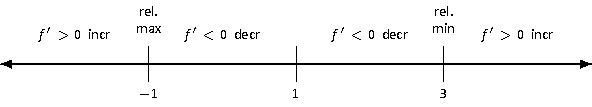
\includegraphics{figures/figincrline2}
%\captionsetup{type=figure}%
%\caption{Number line for $f$ in Example \ref{ex_incr2}.}\label{fig:incrline2}
\end{example}